\section{Parameters identification}
\label{sec:parameters_identification}

In this section, we are going to explain the procedure followed to identify the parameters of the system starting from the FRFs obtained in the previous section.
Basically we are going to simulate an `Operational Modal Analysis' (OMA), even if in this case we already have the exact model of the system.

In particular, we know that for a multi degree-of-freedom system, with lightly damped modes and in particular in case of well distinguished peaks, the FRF can be approximated around a given natural frequency $\omega_n$ as:

\begin{equation}
    H{j, k}^{NUM}(\Omega) = \frac{A_{j, k}^(i)}{-\Omega^2 + 2 \xi_i \omega_i \Omega + \omega_i^2} + \frac{R_{j, k}^L}{\Omega^2} + R_{j, k}^{H} \quad \text{for} \quad \Omega_{min} \leq \omega_i \leq \Omega_{max}
    \label{eq:FRF_approximation}
\end{equation}

As we can see, the FRF is approximated as a sum of three terms: a second order term, a low frequency term and a high frequency term.
The second order term is the one that we are interested in, since it is the one that contains the information about the natural frequency and the damping ratio of the system.
However, if the peaks are not well distinguished, the low and high frequency terms can interfere with the second order term and became non-negligible in the approximation.

In the following, a common procedure is explained to identify all the unknown parameters of $H{j, k}^{NUM}(\Omega)$, once the experimental FRFs are available.
In particular, we will see how to identify the natural frequencies $\omega_i^{NUM}$, the damping ratios $\xi_i^{NUM}$, and the gains $A_{j, k}^{NUM}$, $R_{j, k}^L$ and $R_{j, k}^H$, using minimization techniques.


\subsection{Procedure}
\label{subsec:procedure}

Many of the following steps are based on the assumption that the frequencies vector defining the FRFs, has a higher enough resolution to properly address the following procedure.
In case of a low resolution, the frequencies vector should be at least interpolated in order to obtain a more fine grid over the frequency range of interest.

All the following steps, must be repeated for each natural frequency $\omega_i$ of the system.

\paragraph{Natural frequencies}

The first step is to identify the value of the natural frequency $\omega_i^{NUM}$ of the system.

This can be done by looking at the peaks of the FRFs.
If we have many FRFs at our disposal (for example, we have many sensors or we have performed many tests), we can average the FRFs in order to reduce the noise and obtain a more reliable result.
Remember that the natural frequency identified has to be the same for all the FRFs.

\paragraph{Damping ratios}

The second step is to identify the value of the damping ratio $\xi_i^{NUM}$ of the system.

For this purpose, we can use both the `phase derivative' method or the `half power bandwidth' method (also known as `peak picking' method).

For this assignment, we decided to use the `phase derivative' method, given that the experimental FRFs have a fine enough grid of frequencies.

By looking at the phase of the FRF evaluated at the natural frequency $\omega_i$, we observe that the slope of the phase can be directly related to the damping ratio $\xi_i$.
In particular:

\begin{equation}
    \frac{\partial \angle H_{j, k}(\Omega)}{\partial \Omega} \biggl|_{\Omega = \omega_i} = - \frac{1}{\xi_i \omega_i}
    \label{eq:phase_derivative}
\end{equation}

Based on this relation, we can isolate the damping ratio $\xi_i$ and obtain its value numerically, computing the derivative of the phase of the FRF evaluated at the natural frequency $\omega_i$ using a finite difference method.

\begin{equation}
    \xi_i^{NUM} = - \frac{1}{\omega_i^{NUM} \cdot \frac{\Delta \angle G_{i,k}^{NUM}(\omega_i^{NUM})}{\Delta \omega}}
\end{equation}

\paragraph{Gain $A_{j, k}^{NUM}$}

The third step is to identify the value of the gain $A_{j, k}^{NUM}$ of the system.

This can be done by looking at the magnitude of the FRFs evaluated at the natural frequency $\omega_i$.
In particular, we can obtain the value of the gain $A_{j, k}^{NUM}$ numerically as:

\begin{equation}
    A_{j, k}^{NUM} = 2 \left| G_{j, k}^{EXP}(\omega_i^{NUM}) \right| \omega_i^2 \xi_i^{NUM}
\end{equation}

\paragraph{Final minimization algorithm}

Finally, we can proceed with the minimization of the error between the experimental FRFs and the model FRFs, in order to identify the `exact' values of all the parameters of the system, since the previous steps are only needed as a first approximation.

To do so, we define the error function as:

\begin{equation}
    \epsilon = \sum_{j, k, \Omega} \left| H_{j, k}^{NUM}(\Omega) - H_{j, k}^{EXP}(\Omega) \right|^2
    \label{eq:error_function}
\end{equation}

Which we can think of as the sum of the squared differences between the experimental FRFs and the numerical FRFs evaluated at all the considered frequencies around the analyzed natural frequency $\omega_i$.

In order to minimize the error function, we can use a minimization algorithm, such as the `Levenberg-Marquardt' algorithm, which is a combination of the `Gauss-Newton' algorithm and the `Steepest Descent' algorithm.
This algorithm is particularly useful in case of non-linear least squares problems, such as the one we are facing.

In \texttt{MATLAB}, the `Levenberg-Marquardt' algorithm is implemented in the function \texttt{lsqnonlin}.

\subsection{Parameters identification results}
\label{subsec:parameters_identification_results}

Once the previously explained procedure has been applied to all the natural frequencies of the system (consider for each one, every experimental FRFs at our disposal), we can reassemble the identified parameters so to compute the numerical FRFs of the system based on Equation \ref{eq:FRF_approximation}.

In the following figures, the result obtained considering the FRF relative to an input in $x_k = 1.0m$ and an output in $y_j = 0.6m$ is shown.

\begin{figure}[H]
    \centering
    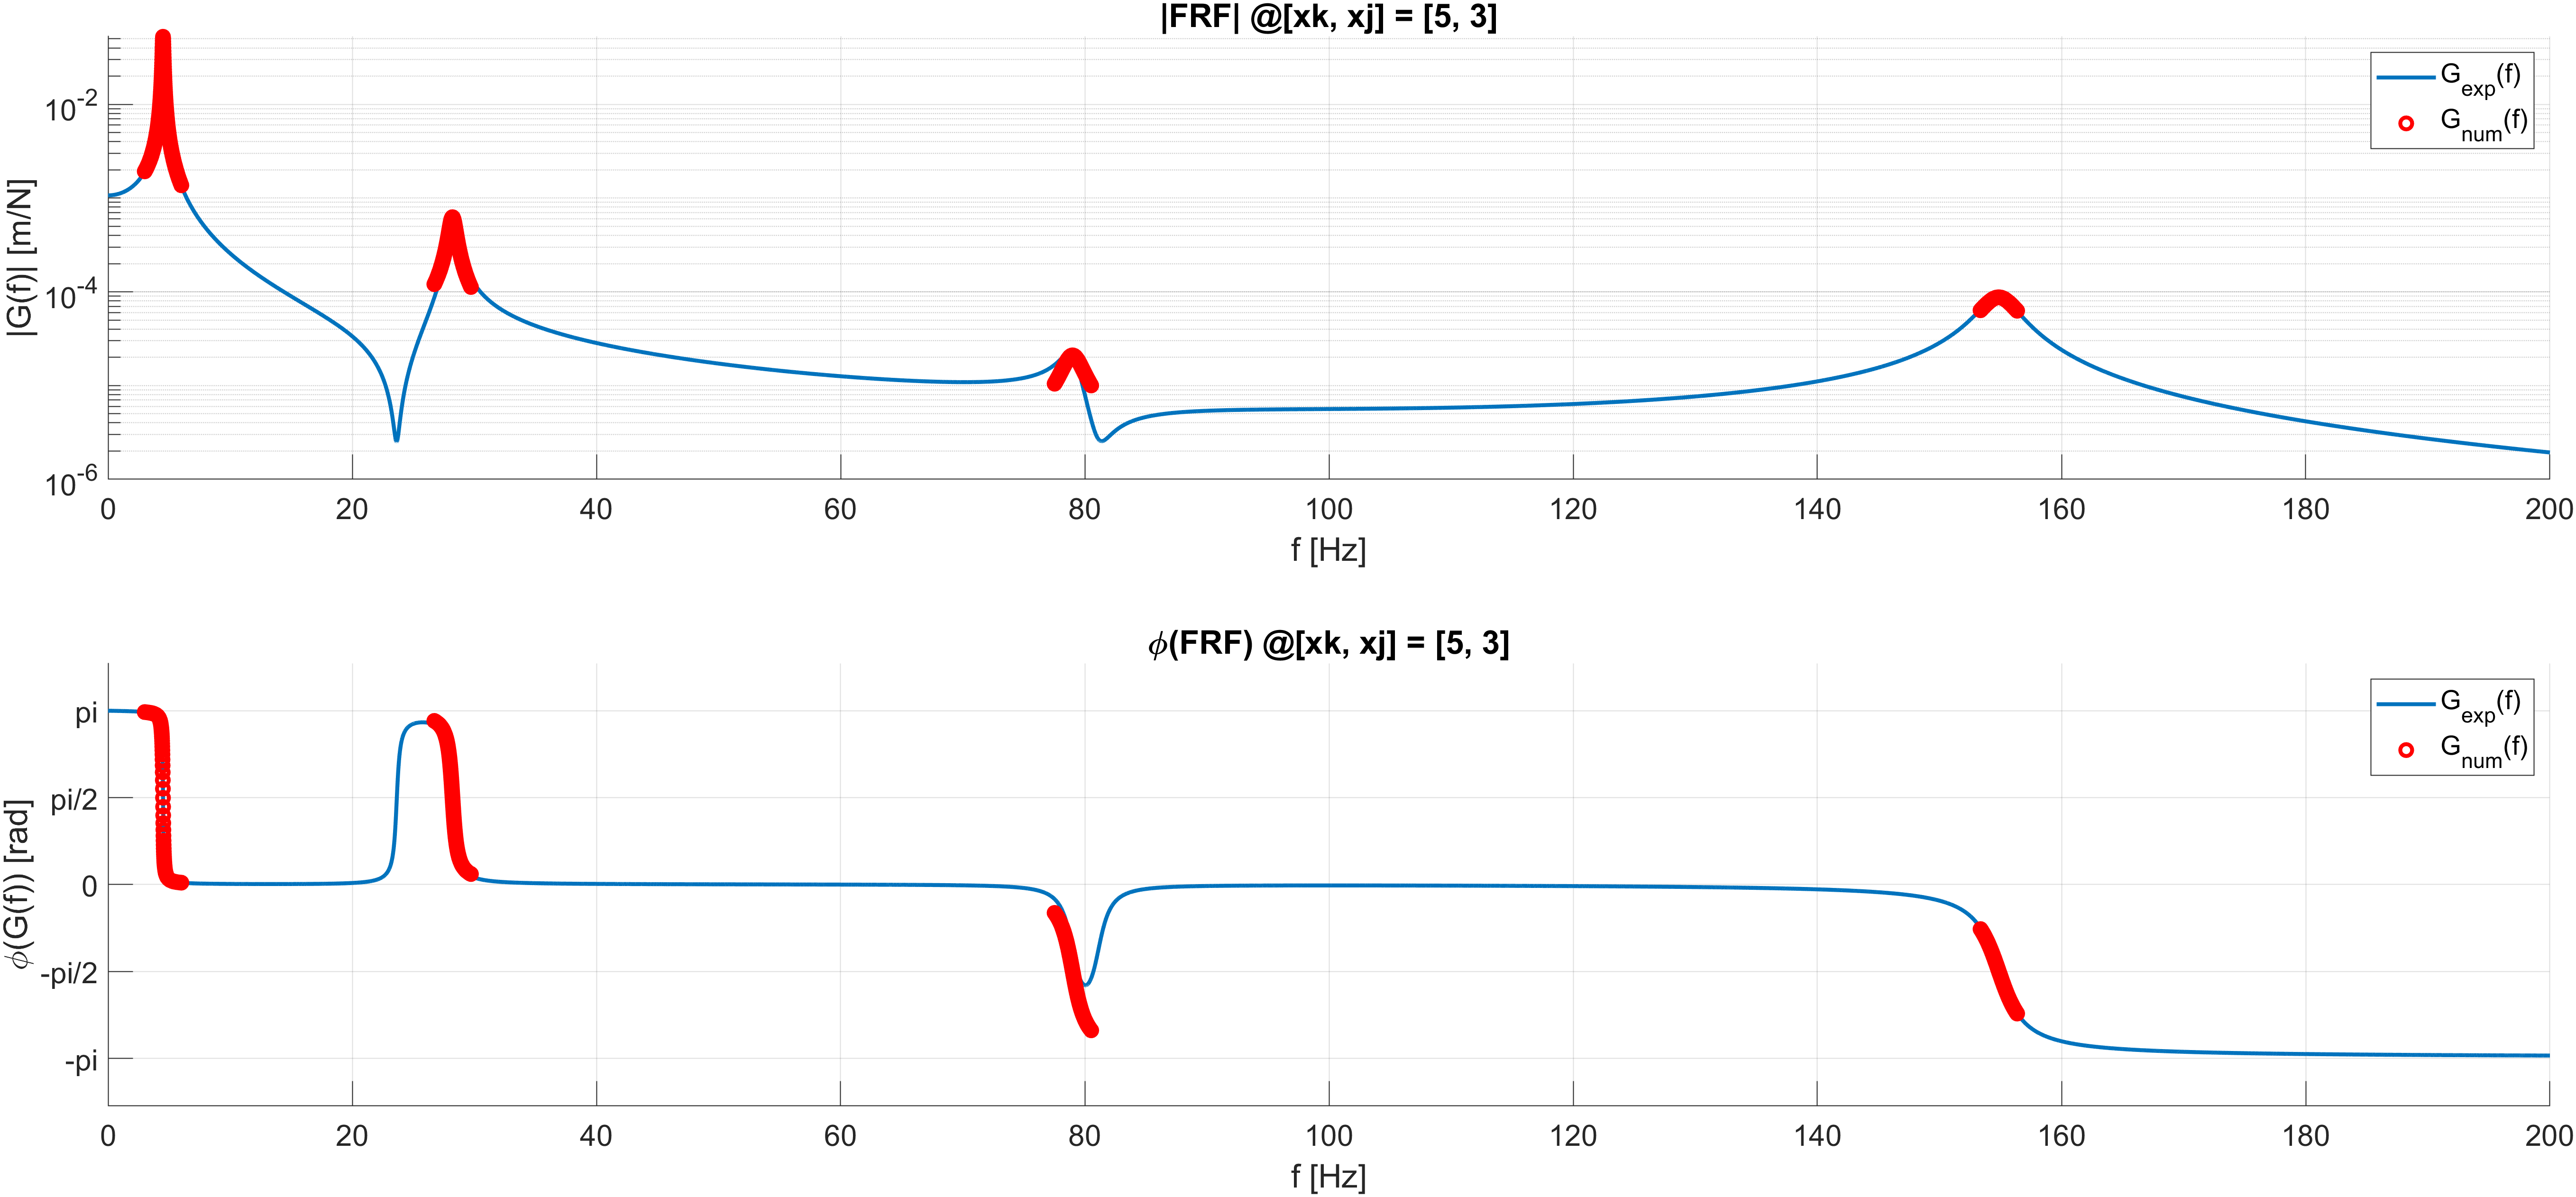
\includegraphics[width=\textwidth]{img/MATLAB/Part_A/Comparison_FRF_couple_3_5.png}
    \caption{FRF identification for $x_k = 1.0m$ and $y_j = 0.6m$}
    \label{fig:FRF_identification}
\end{figure}

\begin{figure}[H]
    \begin{minipage}[b]{0.45\textwidth}
        \centering
        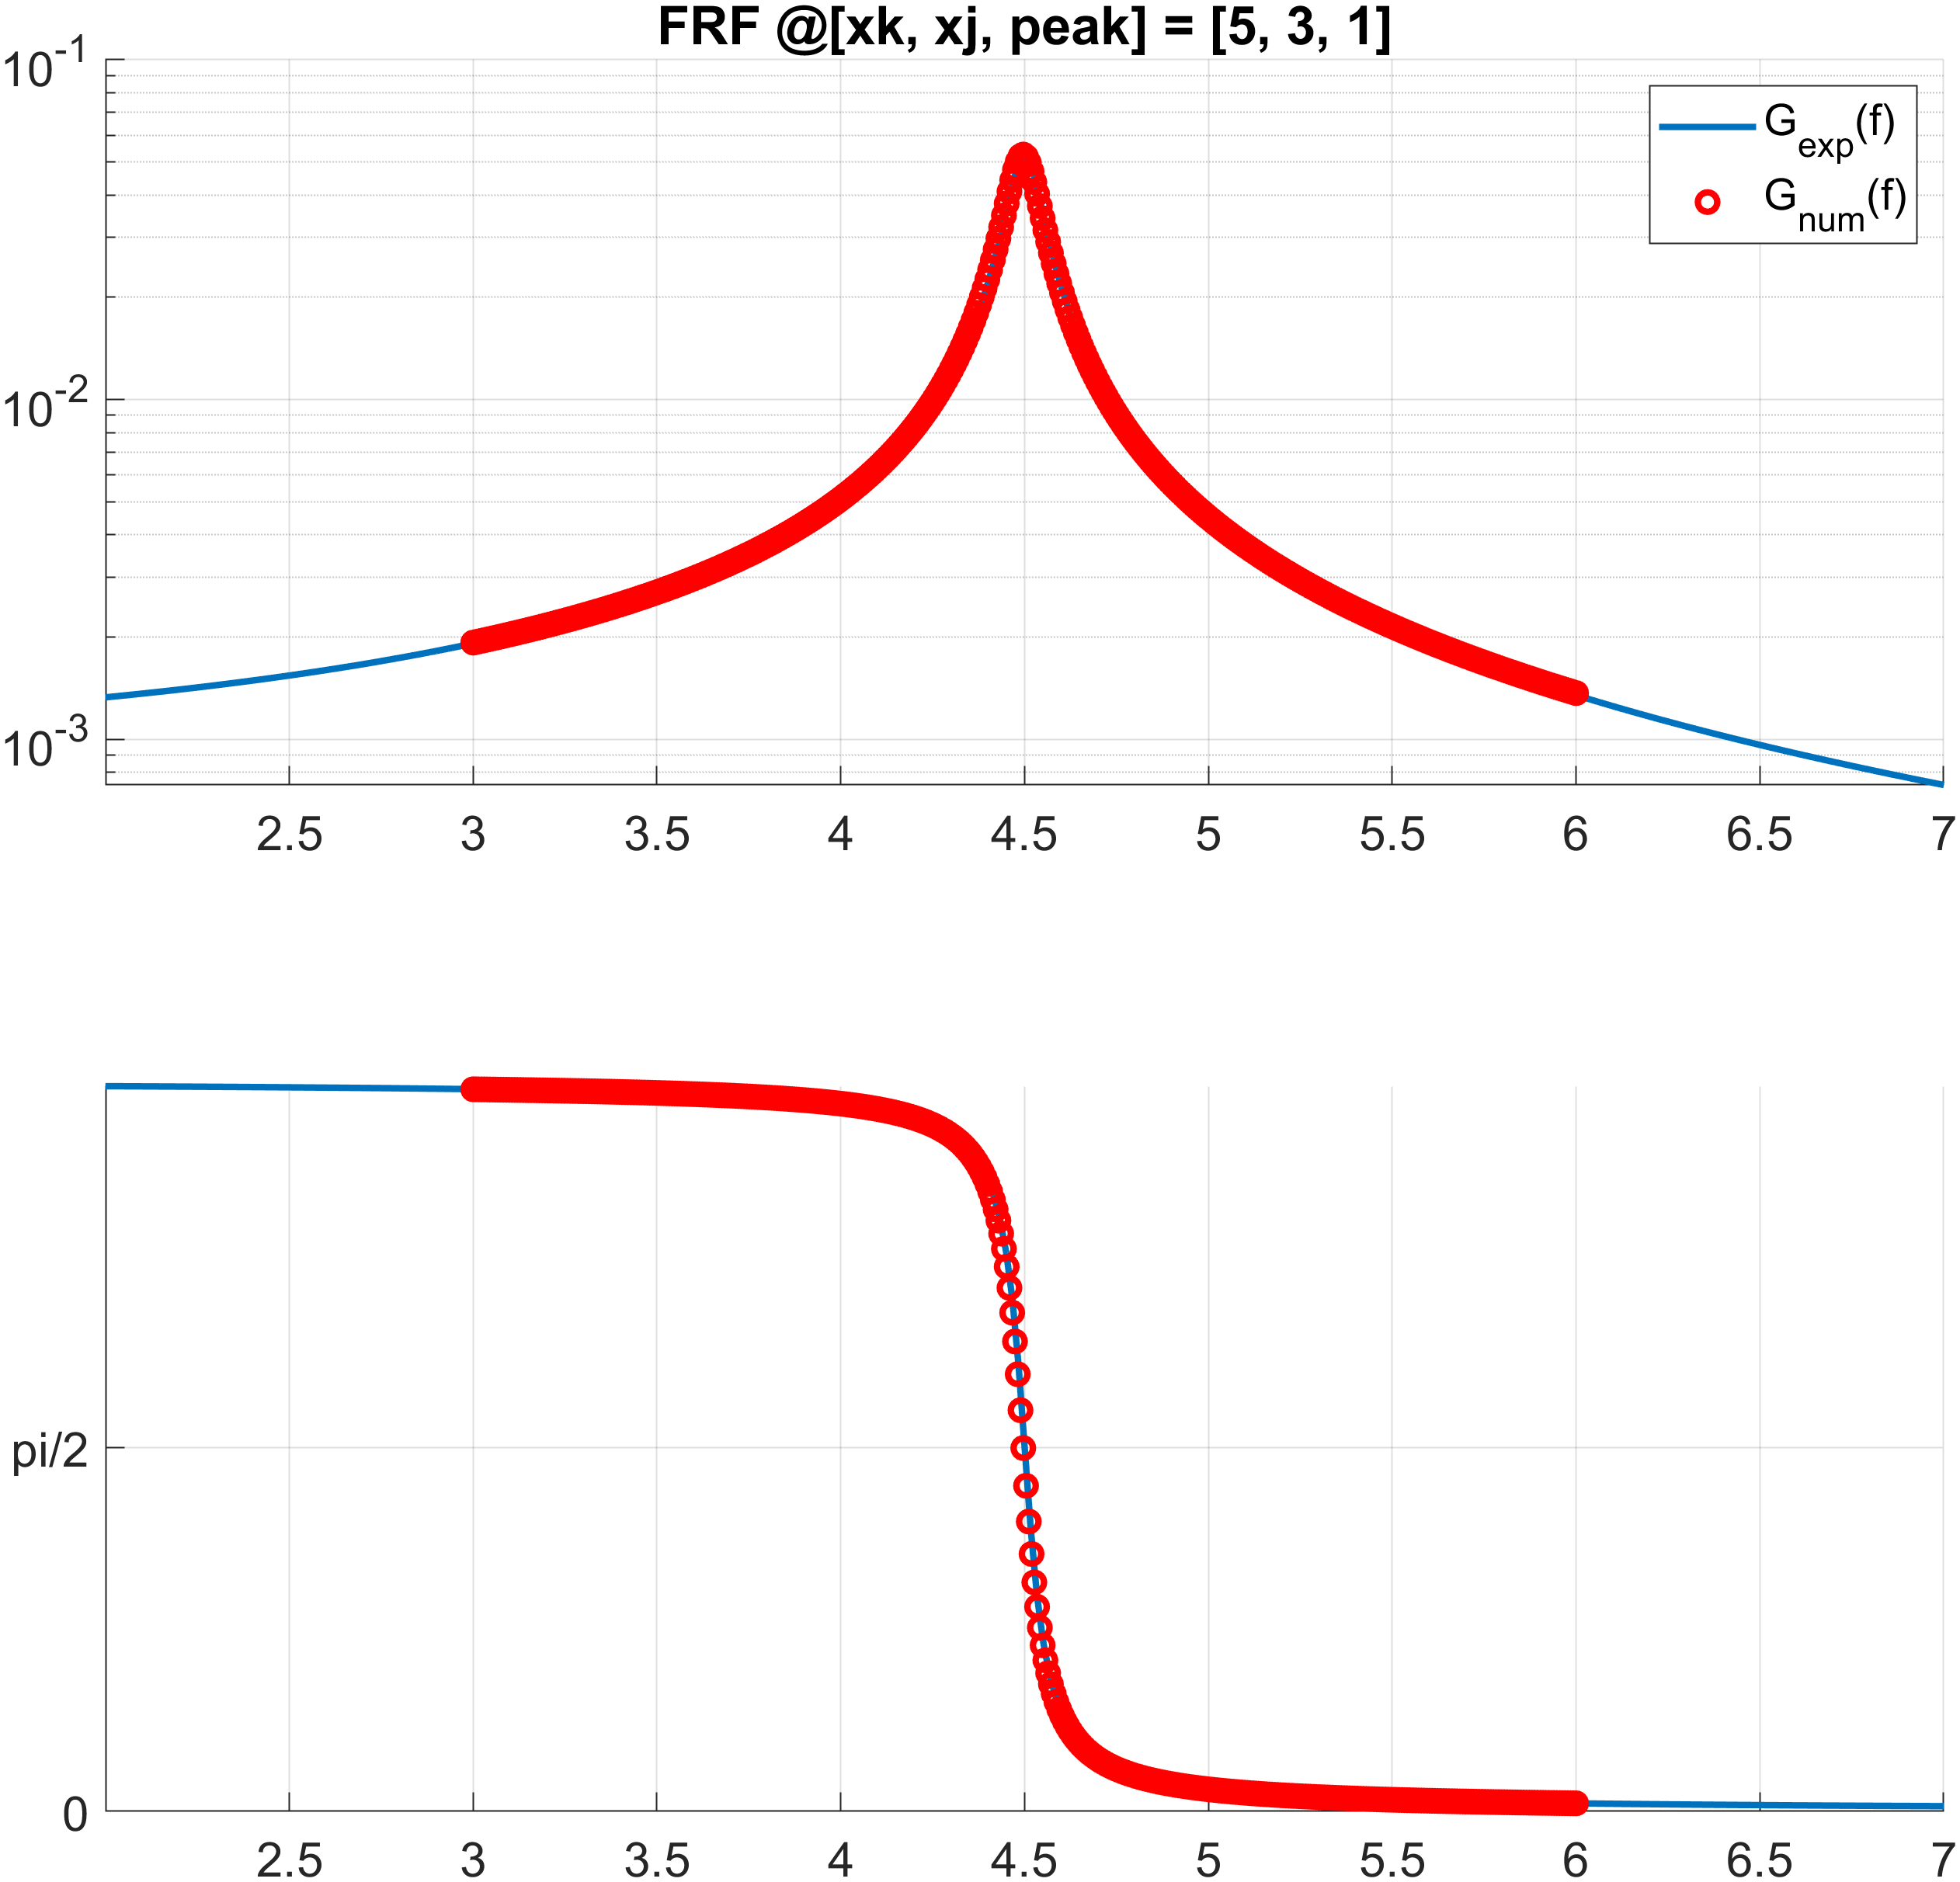
\includegraphics[width=\textwidth]{img/MATLAB/Part_A/Comparison_FRF_couple_3_5_zoom_peak_01.png}
    \end{minipage}
    \hfill
    \begin{minipage}[b]{0.45\textwidth}
        \centering
        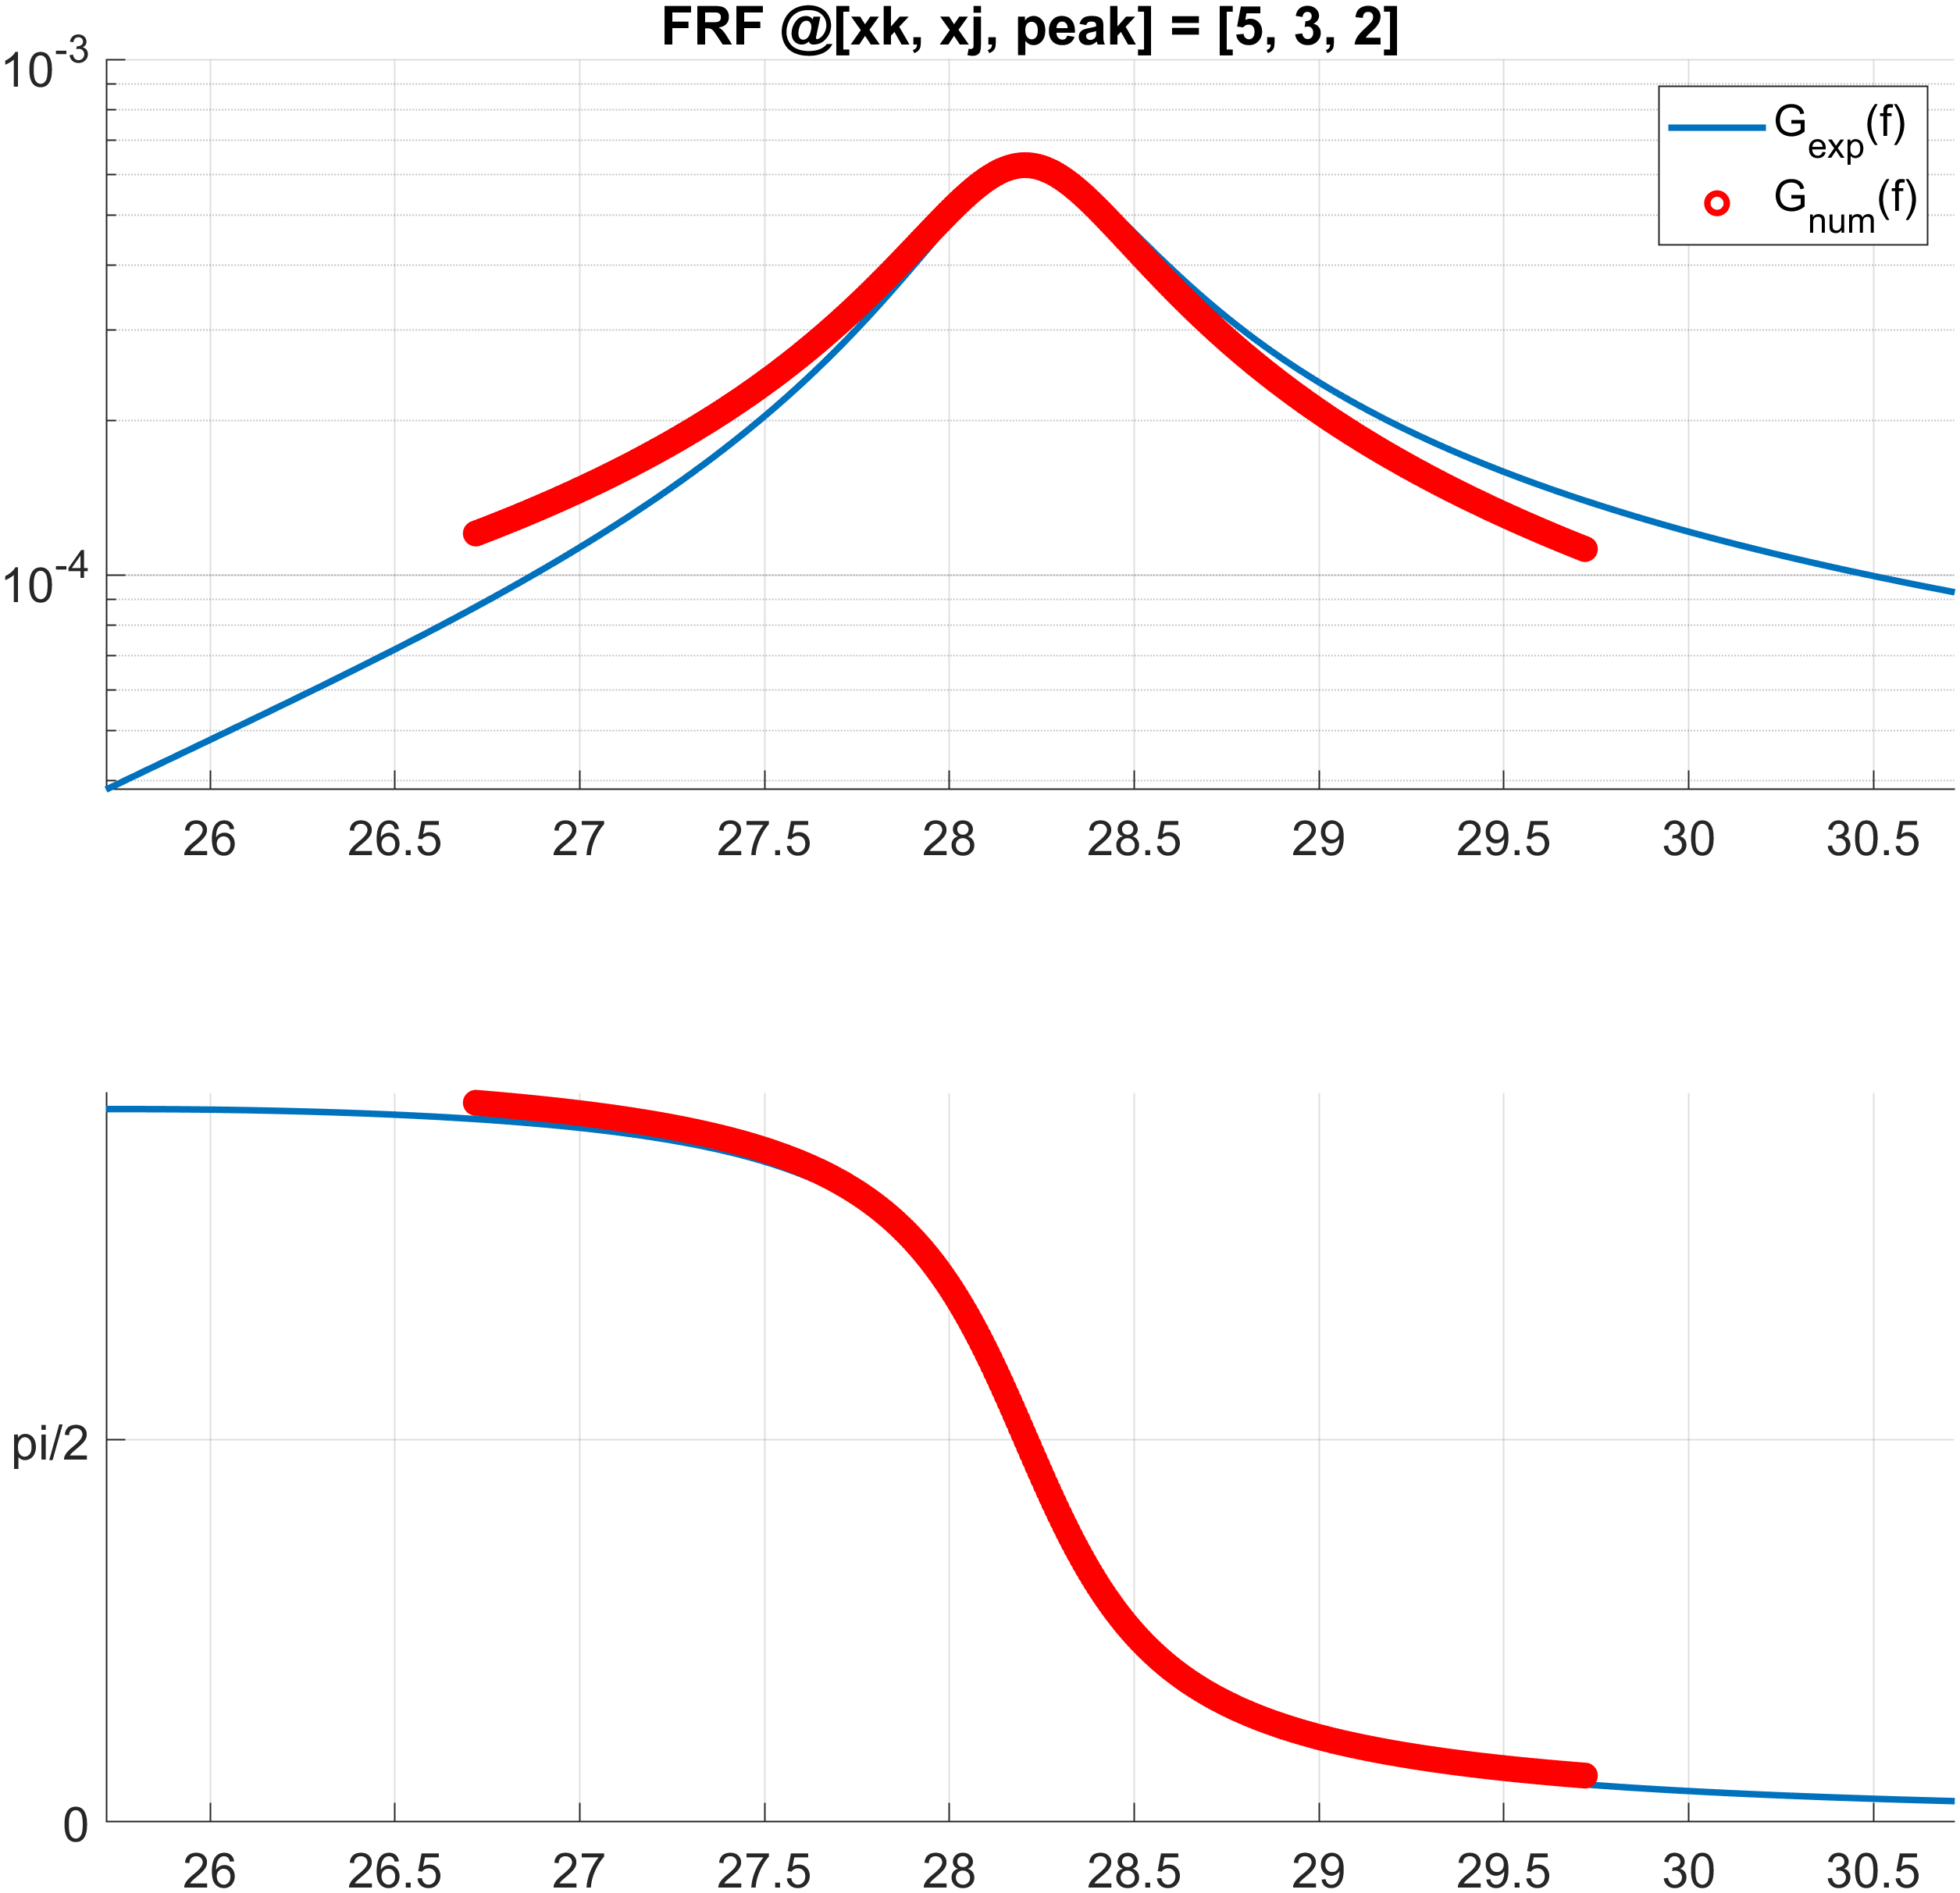
\includegraphics[width=\textwidth]{img/MATLAB/Part_A/Comparison_FRF_couple_3_5_zoom_peak_02.png}
    \end{minipage}
    \begin{minipage}[b]{0.45\textwidth}
        \centering
        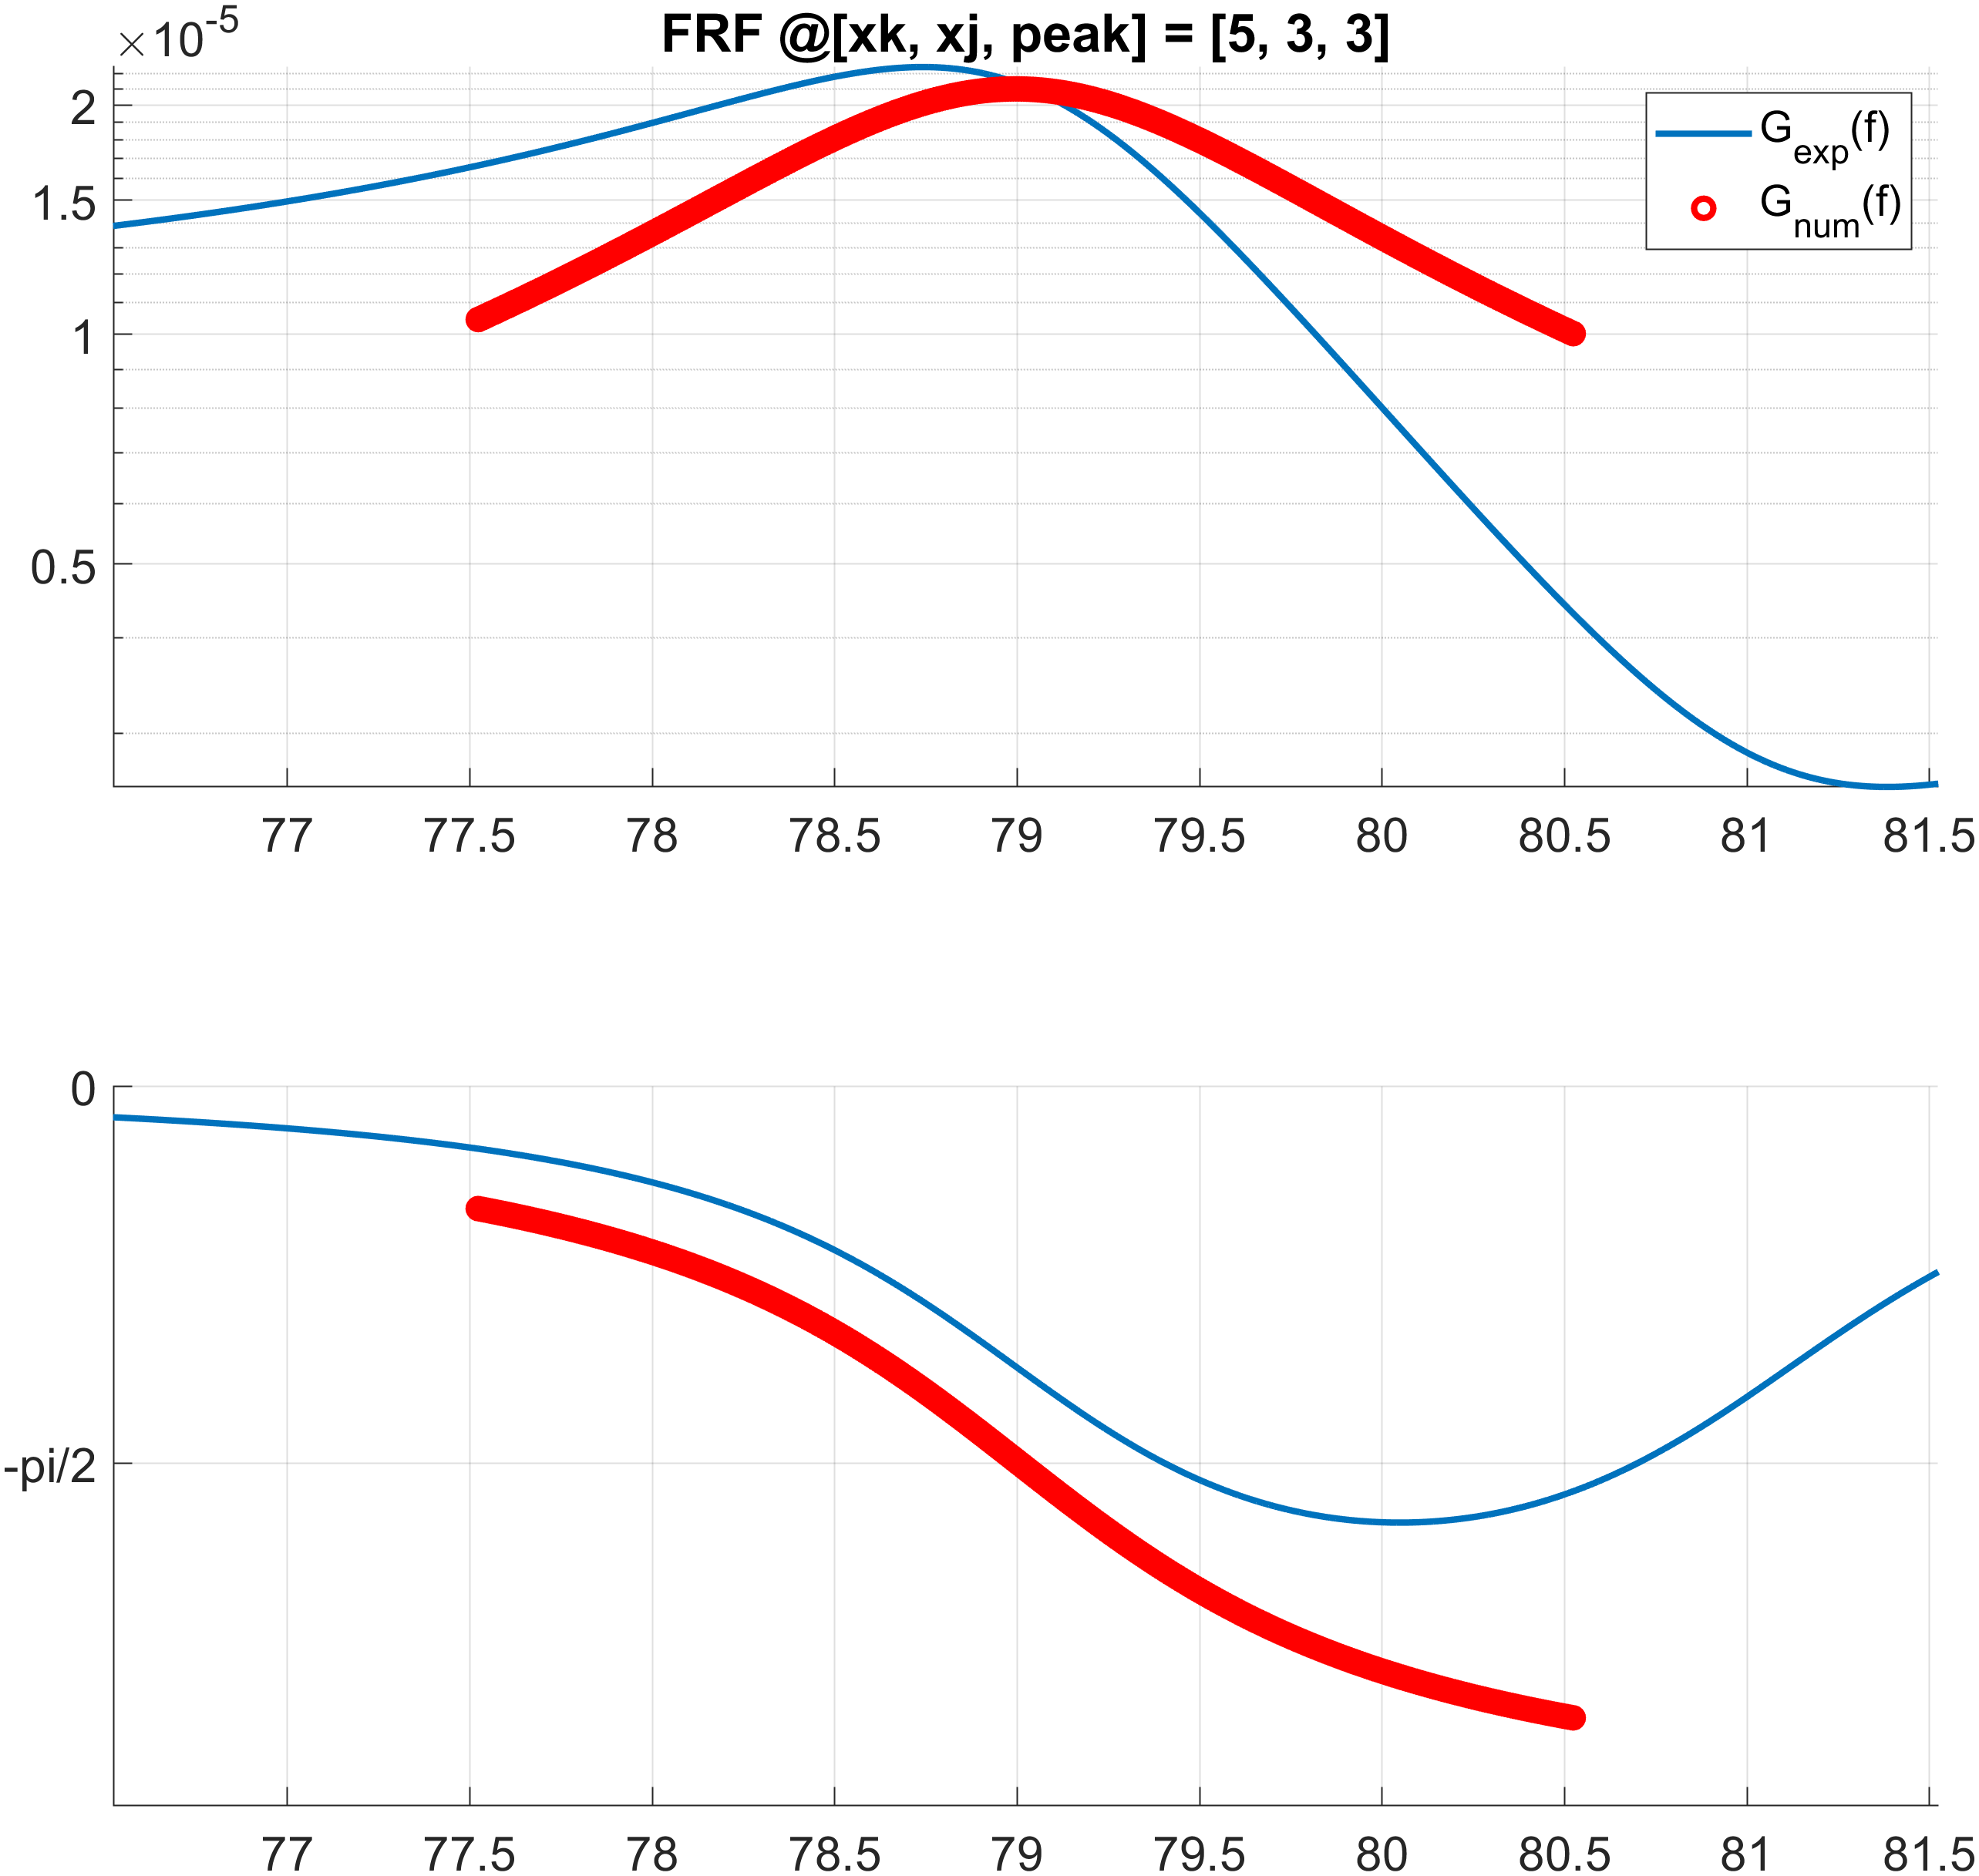
\includegraphics[width=\textwidth]{img/MATLAB/Part_A/Comparison_FRF_couple_3_5_zoom_peak_03.png}
    \end{minipage}
    \hfill
    \begin{minipage}[b]{0.45\textwidth}
        \centering
        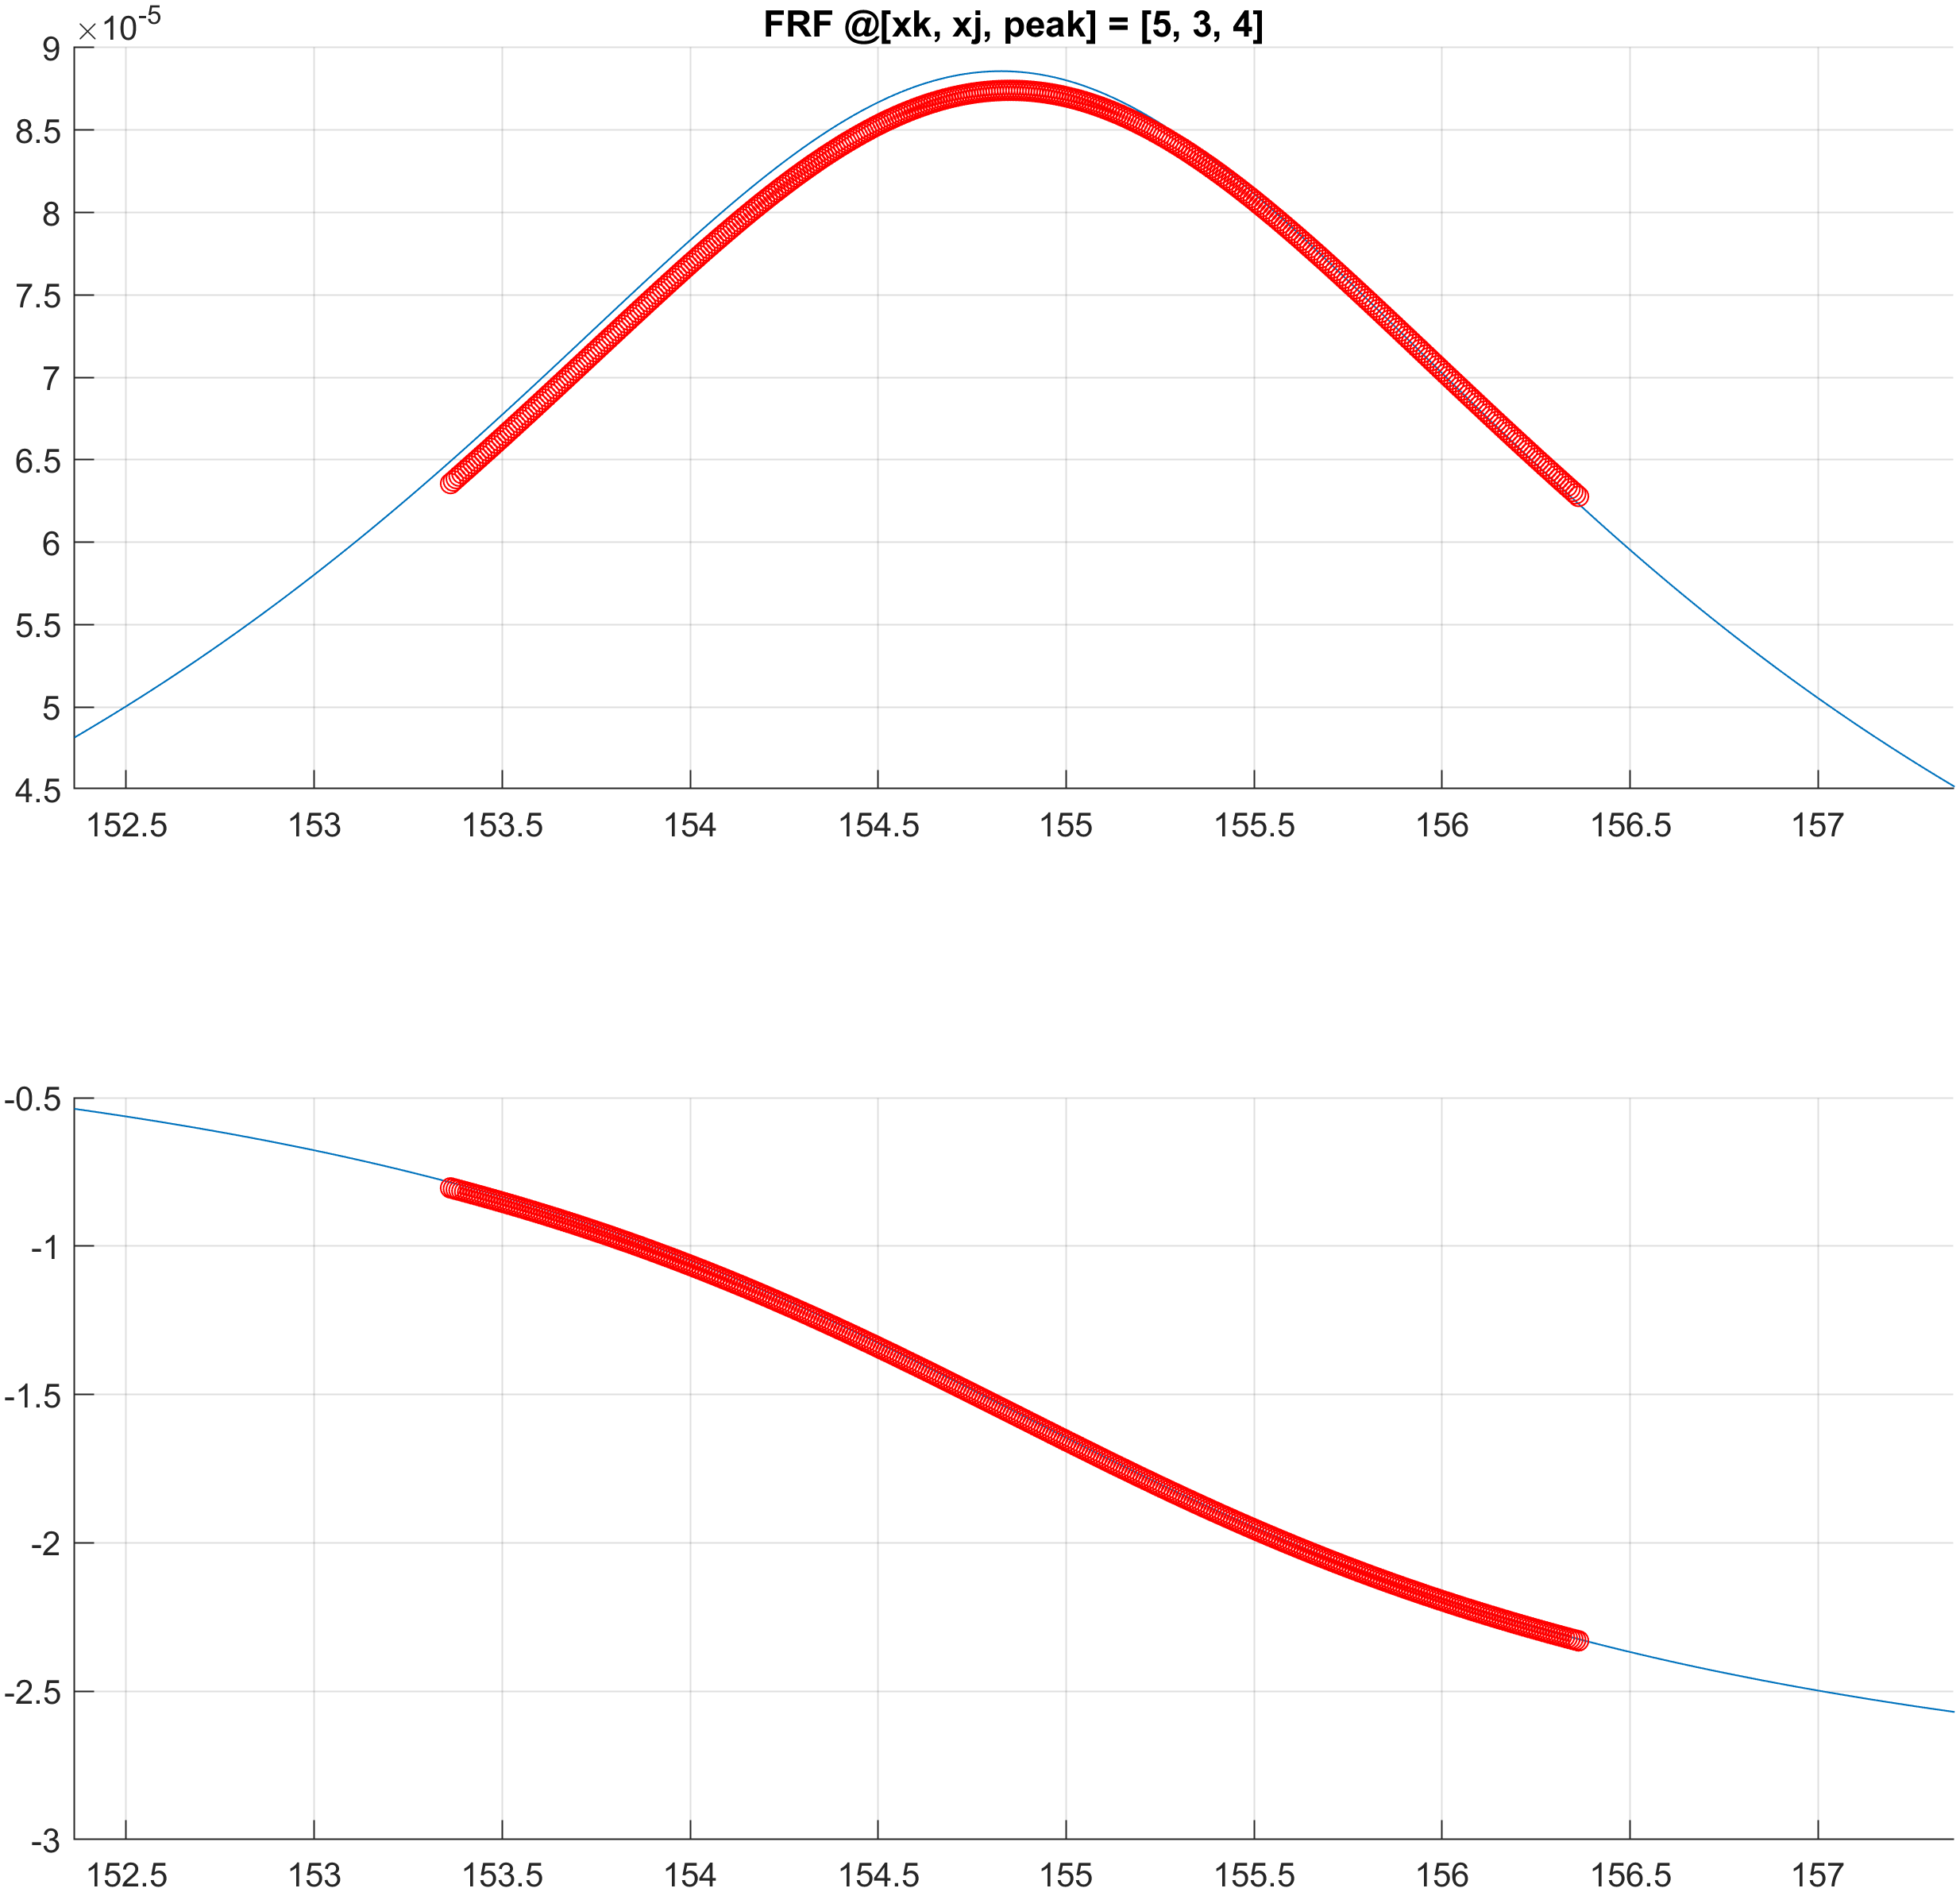
\includegraphics[width=\textwidth]{img/MATLAB/Part_A/Comparison_FRF_couple_3_5_zoom_peak_04.png}
    \end{minipage}
    \caption{Zoom over the peaks of the FRF identification for $x_k = 1.0m$ and $y_j = 0.6m$}
    \label{fig:FRF_identification_zoom}
\end{figure}

